%!TEX root = head-full.tex

\section{Partition Function Estimation} \label{sec:rbm}


\subsection{Restricted Bolztmann Machine}
Co-invented and enhanced largely\cite{hinton2006reducing} by Geoff Hinton, a Restricted Bolzmann Machine(RBM)\cite{mcclelland1987parallel} is a model which brings the idea of a physics concept to the field of computer science.

\begin{figure*}[tb]
% \vspace{-0.5in}
  	\centering
  	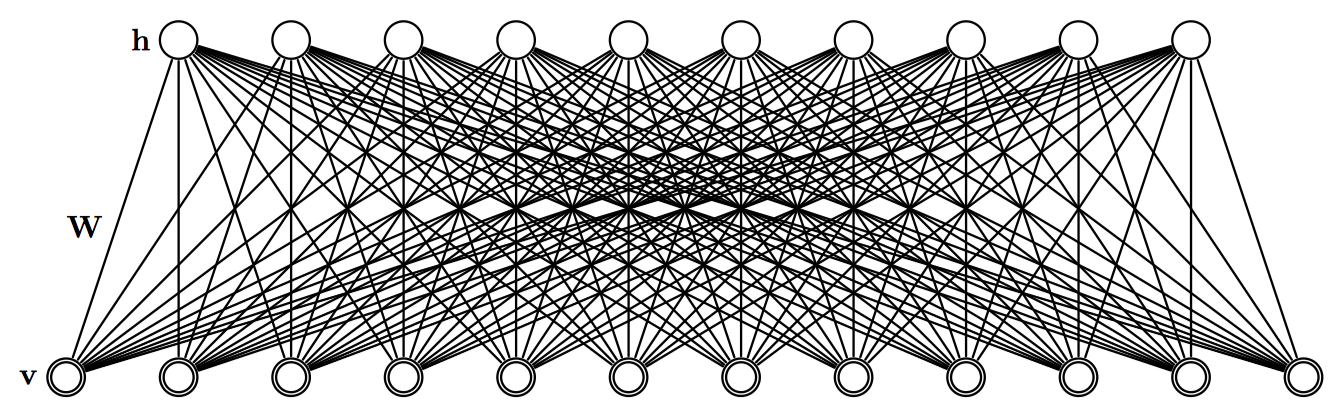
\includegraphics[width=1\textwidth]{figure/rbm.png}
% \vspace{-0.2in}
	\caption{A Restricted Boltzmann Machine}
	\label{fig:rbm}
\end{figure*}

\subsubsection{Introduction}
An RBM is a two-layer undirected model(Figure~\ref{fig:rbm}). The first layer of the RBM is called visible layer, and the second is called the hidden layer. In the model, every visible units are connected to all hidden units and vice versa. For every given value of visible layer $\mathbf v$ \& hidden layer $\mathbf h$, we can define an energy of this state.
\begin{equation}
E(\mathbf v,\mathbf h;\theta)=-\mathbf v^T\mathbf W\mathbf h-\mathbf b^T\mathbf v-\mathbf a^T\mathbf h
\end{equation}
where $\theta =\{W,\mathbf b,\mathbf a\}$ are the model configurations. $W_{ij}$ represents the weight between visible unit $v_{i}$ and hidden unit $h_{j}$. $\mathbf b$ \& $\mathbf a$ are biases for visible and hidden layer, respectively.

\subsubsection{Training an RBM}
On training an RBM, we want our RBM model to have a lowest scale of energy. By doing so, we have to calculate the joint distribution over the visible and hidden units, which is defined by:
\begin{equation}
	p(\mathbf v,\mathbf h;\theta)=\frac{e^{-E(\mathbf v,\mathbf h;\theta)}}{Z(\theta)}
\end{equation}
where
\begin{equation}
	Z(\theta)=\sum_{\mathbf v} \sum_{\mathbf h} e^{-E(\mathbf v,\mathbf h;\theta)}
\end{equation}
is the partition function.

However, calculating partition functions has always been an intractable work since we have to traverse all the possible state of $\mathbf v$ \& $\mathbf h$.
When the model grows large, this process will be very time \& rescouces consuming and thus become unrealistic for the real practice.

So, we have to introduce methods to estimate the partition functions instead of just calculating it in brute force. Although some deviation may include in the estimation, but the efficiency along with them make them preferable. In fact, studies have shown that only few deviation is included that we could just ignore it since it does petty influence on our training.

In the next subsection, we will discuss about three methods available, which each have their pros and cons in doing this complex estimation.



\subsection{Algorithms}

%!TEX root = RBM.tex

\subsubsection{Thouless-Anderson-Palmer Sampling\protect\footnote{Available at \protect\url{https://github.com/lzhbrian/MCMC/blob/master/rbm/TAP.m} in Matlab}}
Thouless-Anderson-Palmer Sampling(TAP)\cite{gabrie2015training} is a very efficient and easy-to-practice iterative procedure based on an improved mean field method from statistical physics called Thouless-Anderson-Palmer approach.

The main idea of this method is to iteratively compute the magnetization vector $m^{v}$,$m^{h}$, and then input the values into the Legendre transform of the free energy $F=log(Z(\theta))$ to compute it.

The Legendre transform of $F$ to the second order is:
\begin{equation}
\begin{split}
\Gamma(\mathbf m^{v},\mathbf m^{h}) &\approx - S(\mathbf m^{v},\mathbf m^{h}) - \sum_{i} a_{i}m^{v}_{i} - \sum_{j} b_{j}m^{h}_{j} \\
& - \sum_{i,j} \Bigg( W_{i,j}m^{v}_{i}m^{h}_{j} \\
& - 0.5W_{ij}\Big(m^{v}_{i}-(m^{v}_{i})^2\Big)\Big(m^{h}_{j}-(m^{h}_{j})^2\Big) \Bigg)
\end{split}
\end{equation}
where $S(\mathbf m^{v},\mathbf m^{h})$ indicates the entropy:
\begin{equation}
\begin{split}
S(\mathbf m^{v},\mathbf m^{h}) &= - \sum_{i} \Bigg(m^{v}_{i}logm^{v}_{i} + (1-m^{v}_{i})log(1-m^{v}_{i}) \Bigg) \\
&- \sum_{j} \Bigg(m^{h}_{j}logm^{h}_{j} + (1-m^{h}_{j})log(1-m^{h}_{j}) \Bigg)
\end{split}
\end{equation}

The pseudo code of this algorithm is shown below:


%!TEX root = RBM.tex

\subsubsection{Annealed Importance Sampling\protect\footnote{Available at \protect\url{https://github.com/lzhbrian/MCMC/blob/master/rbm/AIS.m} in Matlab}}
Annealed Importance Sampling(AIS)\cite{neal2001annealed,salakhutdinov2009learning} is probably one of the most preferable estimating methods avaible.

Previous work \cite{mackay2003information} have shown that if $P_{A}$ and $P_{B}$ in the SIS method is not close enough, the estimator would be very poor.

Based on SIS, the main idea of this algorithm is to gradually alter the value from an known $Z_{A}$ to our required $Z_{B}$ (or $Z_{K}$), by the following identity:
\begin{equation}
\frac{Z_{K}}{Z_{0}} = \frac{Z_{1}}{Z_{0}} \frac{Z_{2}}{Z_{1}} ... \frac{Z_{K}}{Z_{K-1}}
\end{equation}
where 
\begin{equation}
\frac{Z_{K}}{Z_{k+1}} = \frac{1}{M} \sum_{i=1}^{M} \frac{P_{k+1}^{*}(\mathbf x^{(i)})}{P_{k}^{*}(\mathbf x^{(i)})}
~~where~ x^{(i)} \sim P_{k}
\end{equation}
in which we can get $x_{k+1}$ from:
\begin{equation}
\begin{aligned}
p(h^{A}_{j}=1|\mathbf v) &= sigmoid\Bigg( (1-\beta_{k})\Bigg(\sum_{i}W^{A}_{ij}v_{i}+a^{A}_{j}\Bigg) \Bigg) \\
p(h^{B}_{j}=1|\mathbf v) &= sigmoid\Bigg( \beta_{k}\Bigg(\sum_{i}W^{B}_{ij}v_{i}+a^{B}_{j}\Bigg) \Bigg) \\ 
p(v'_{i}=1|\mathbf h) &= sigmoid\Bigg( (1-\beta_{k})\Bigg(\sum_{j}W^{A}_{ij}h_{i}^{A}+b^{A}_{i}\Bigg) \\
& + \beta_{k}\Bigg(\sum_{j}W^{B}_{ij}h_{j}^{B}+b^{B}_{i}\Bigg) \Bigg) 
\end{aligned}
\end{equation}
this procedure is shown in Figure~\ref{fig:xkxk1}.

\begin{figure}[tb]
% \vspace{-0.5in}
  	\centering
  	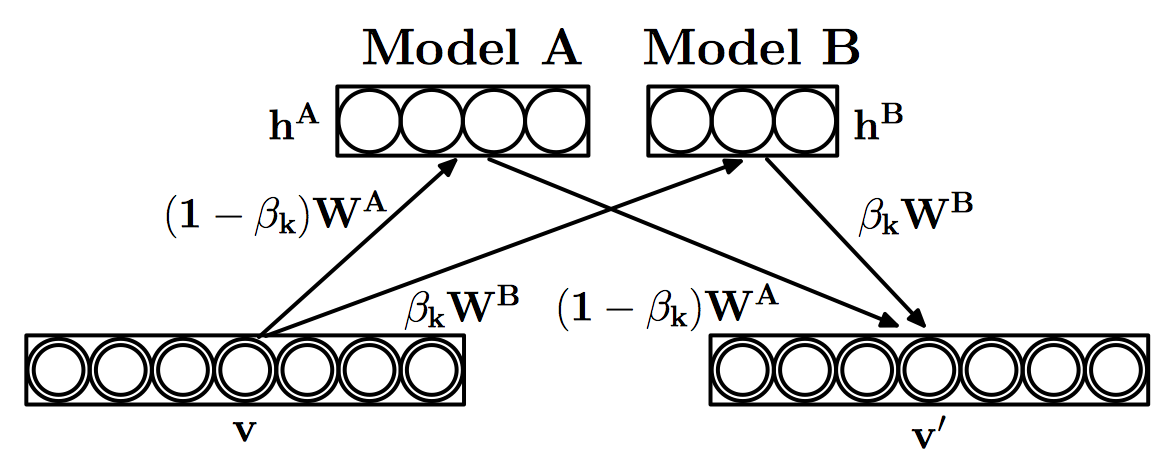
\includegraphics[width=0.4\textwidth]{figure/xkxk1.png}
% \vspace{-0.2in}
	\caption{The transition process from $x_{k}$ to $x_{k+1}$ which leaves $P_{k}(\mathbf v)$ invariant.}
	\label{fig:xkxk1}
\end{figure}

Note that model A indicates an initial model which we can easily compute all its configurations.

$\mathbf \beta$ in the above equations is defined by users as a set of inverse temperatures $\{0= \beta_{1} < \beta_{2} < ... < \beta_{K} =1\}$, which can define a sequence of
\begin{equation}
P_{k}(\mathbf x) \propto P_{A}^{*}(\mathbf x)^{1-\beta_{k}} P_{B}^{*}(\mathbf x)^{\beta_{k}}
\end{equation}
where 
\begin{equation}
P^{*}_{k}(\mathbf v)=\sum_{h^{A}h^{B}}e^{(1-\beta_{k})E(\mathbf v, \mathbf h^{A};\theta_{A})+\beta_{k}E(\mathbf v,\mathbf h^{B};\theta_{B})}
\end{equation}


The pseudo code of this algorithm is shown below:


%!TEX root = RBM.tex

\subsubsection{Rao-Blackwellized Tempered Sampling\protect\footnote{Available at \protect\url{https://github.com/lzhbrian/MCMC/blob/master/src/partition/RTS.m} in Matlab}}

\para{Algorithm}
Similar to AIS, Rao-Blackwellized Tempered (RTS)\cite{carlson2016partition} Sampling also has a set of inverse temperatures $\{0= \beta_{1} < \beta_{2} < ... < \beta_{K} =1\}$, which can define a sequence of
\begin{equation}
f_{k}(\mathbf x) \propto f(\mathbf x)^{\beta_{k}} p_{1}(\mathbf x)^{1-\beta_{k}}
\end{equation}

Different from AIS, we do not traverse $\mathbf \beta$. Instead we sample a $\beta^{*}$ every loop, from the $\mathbf \beta$ set with the distribution $(\beta|x)$.

Subsequently, we sample from $x_{k}$ to $x_{k+1}$ by the probability of $q(x|\beta^{*})$ just like what we did in AIS, shown in Figure~\ref{fig:xkxk1}. However, what also different from AIS is that, we have to iterate from $x_{k}$ to $x_{k+1}$ many times(i.e. 50 times in\cite{carlson2016partition} ) for the sake of getting a better $x_{k+1}$.

At the last of every loop, we update the lower variance estimator $\hat{\mathbf c}$ by
\begin{equation}
\hat{c}_{k} = \hat{c}_{k} + \frac{1}{N}q(\beta_{k}|x)
\end{equation}

Finally, we get $Z_{k}$ by
\begin{equation}
\hat{Z}_{k}^{RTS} = \hat{Z}_{k}\frac{r_{1}\hat{c}_{k}}{r_{k}\hat{c}_{1}},~~k=2,...,K
\end{equation}
in which what we do care is $Z_{B} \approx \hat{Z}_{K}^{RTS}$.

The posterier distribution $q(\beta_{k}|x)$ in the above equations is defined by:
\begin{equation}
q(\beta_{k}|x) = \frac{f_{k}(x)r_{k}/\hat{Z}_{k}}{\sum_{k'=1}^{K} f_{k'}(x)r_{k'}/\hat{Z}_{k'}}
\end{equation}

\para{Practice}
In the paper\cite{carlson2016partition}, Carlson et al. note an initializing method to initialize $Z_{k}$, whose procedure is just like the above process. The only difference is that they sampled $\beta_{k}$ by uniform distribution in every loop, not by the distribution $(\beta|x)$. They claim that after doing such initializing work, then we conduct the algorithms above would acquire a better result.

In our real practice, we directly use the initializing method mentioned above by selecting $\beta_{k}$ with a uniform distribution in every loop. We also initialize the value of $Z_{A}$ by the method we have mentioned in the AIS section using the dataset. And we have found that the result is already satisfying, there is no need to conduct more loops with $\beta_{k}$ sampled by $(\beta|x)$.

Also, we found that we have to conduct the procedure above for several times s.t. we can acquire our desired partition function value.(i.e. We did it for 100 times, that is to say we update $\mathbf Z$ for 100 times).

	\begin{algorithm}
        \caption{Rao-Blackwellized Tempered Sampling}
        \begin{algorithmic}
        	\Require $\{\beta_{k},r_{k}\}_{k=1,...,K}$
            \State Initialize $b_{A}$ by dataset
        	\State Initialize $log \hat{Z}_{k}, k=2,...,K$ 
            \For{$n = 1 \to Runtime$}
            	\State Initialize $\beta \in \{\beta_{1}...\beta_{K}\}$
            	\State Initialize $\hat{c}_{k}=0, k=1,...,K$
                \For{$t = 1 \to N$}
                    \For{$t = 1 \to Transition time$}
                        \State Sample $\mathbf x_{k+1}$ given $\mathbf x_{k}$ using $q(x|\beta^{*})$
                    \EndFor
                    \State $\mathbf x^{*} \gets \mathbf x_{k+1}$
    	            \State Sample $\beta^{*} \sim (\beta|\mathbf x^{*})$ or $\beta^{*} \in \{\beta_{1}...\beta_{K}\}$
    	            \State Update $\hat{c}_{k} \gets \hat{c}_{k}+\frac{1}{N} q(\beta_{k}|\mathbf x^{*})$
    			\EndFor
                \State Update $\hat{Z}^{RTS}_{k} \gets \hat{Z}_{k}\frac{r_{1}\hat{c}_{k}}{r_{k}\hat{c}_{1}}, k=2,...,K$
            \EndFor
        \end{algorithmic}
    \end{algorithm}


\subsubsection{Other methods}
There are many other methods which can also estimate the partition functions. Such as Self-adjusted mixture sampling(SAMS)\cite{tan2015optimally} proposed a method to estimate multiple partition functions together to improve the efficiency. As the length \& time limit, we only implement 3 methods here in this paper.

%!TEX root = RBM.tex

\subsection{Estimating Results}

We estimate the results of the three algorithms using 4 models with 10, 20, 100, 500 hidden units respectively, all 4 models have 784 visible units. The models are trained by the MNIST handwritten digit dataset\cite{lecun1998mnist}.

Note that we only calculate the real value of the partition function in the model with 10 hidden units ($logZ(\theta)=226.11$), due to my poor laptop has broken down several times when calculating the model with 20 hidden units and maltab doesn't even allow to calculate the other two models because they require unimaginable quantity of memories.

\para{AIS}
\begin{table}[t]
\centering
{\small
\begin{tabular}{c|ccc}
    \hline
    \textbf{Hid Units} & \textbf{Mean $logZ(\theta)$} & \textbf{+/-3 sd} & \textbf{Real Value} \\ 
    \hline
	   10  & 226.05 & 0.1762 & 226.11 \\
	   20  & 221.11 & 0.2329 & N/A 	  \\
	   100 & 348.45 & 0.2460 & N/A 	  \\
	   500 & 463.25 & 0.3790 & N/A 	  \\ \hline
\end{tabular}
}
\vspace{-0.1in}
\caption{AIS result (with $\mathbf b$ init) with $+/-3$ standard deviations}
\label{tab:aisresult}
% \vspace{-0.05in}
\end{table}
By setting $\mathbf \beta$ uniformly sampling from 0 to 1 for 10,000 points, we run 100 times of AIS, and get a result with $+/-3$ standard deviations (Table~\ref{tab:aisresult}). In a model with 10 hidden units. We see AIS with init almost obtain the real value (226.11) without error.

\begin{figure}[t]
	\centering
	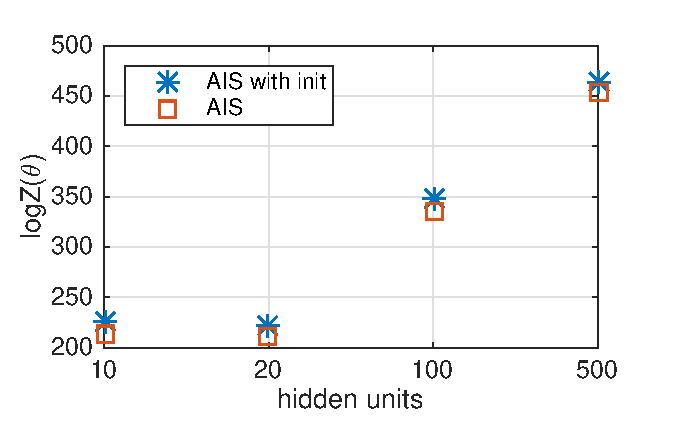
\includegraphics[width=0.48\textwidth]{figure/AIS_results/ais_result.eps}
% \vspace{-0.1in}
	\caption{Comparison of AIS method, with or without an initialization of $\mathbf b$}
\label{fig:aisinit} % FIG1
\end{figure}
From Figure~\ref{fig:aisinit}, we can see that the estimation results will differ a lot if we use an initialization method to initialize the visible bias $\mathbf b$, as mentioned in the previous subsection. And from the validation of the 10 hidden units case, we can infer that with a initialization of $\mathbf b$ would largely improve the result.




\para{RTS}
When doing the practice of RTS, as mentioned in the last subsection, we directly use the initializing method mentioned above by selecting $\beta_{k}$ with a uniform distribution in every loop. Also, we use the same initialization method as in AIS to initialize $\mathbf b$ in model A. 

We make 50 transitions from $x_{k}$ to $x_{k+1}$ in every loop, we take 100 loops (i.e.$N=100$) every time, and we conduct the whole procedure for 100 times (i.e.we update $\mathbf Z$ for 100 times). Also, we select 100 point of $\mathbf \beta$ uniformly sampled from 0 to 1. 

By conducting the whole above procedure for 20 times, we can obtain a result which is as good as AIS (Table~\ref{tab:allresult}). However, the efficiency of RTS show weaker performance than that of AIS (Table~\ref{tab:efficiencyresult}).

\para{TAP}
\begin{figure}[t]
\begin{minipage}[t]{1\linewidth}
	\centering
  	\subfigure{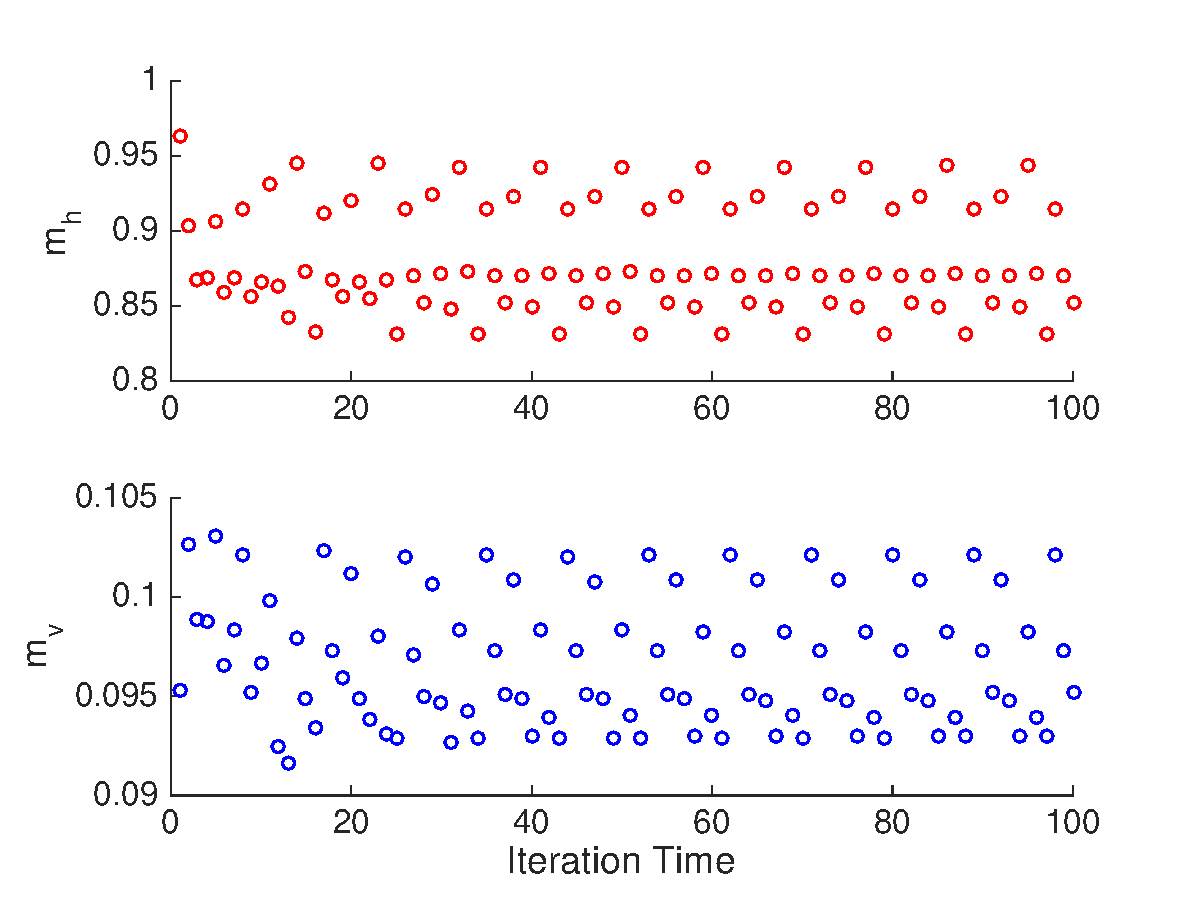
\includegraphics[width=0.48\textwidth]{figure/TAP_results/mvmh_10.eps}}
	\subfigure{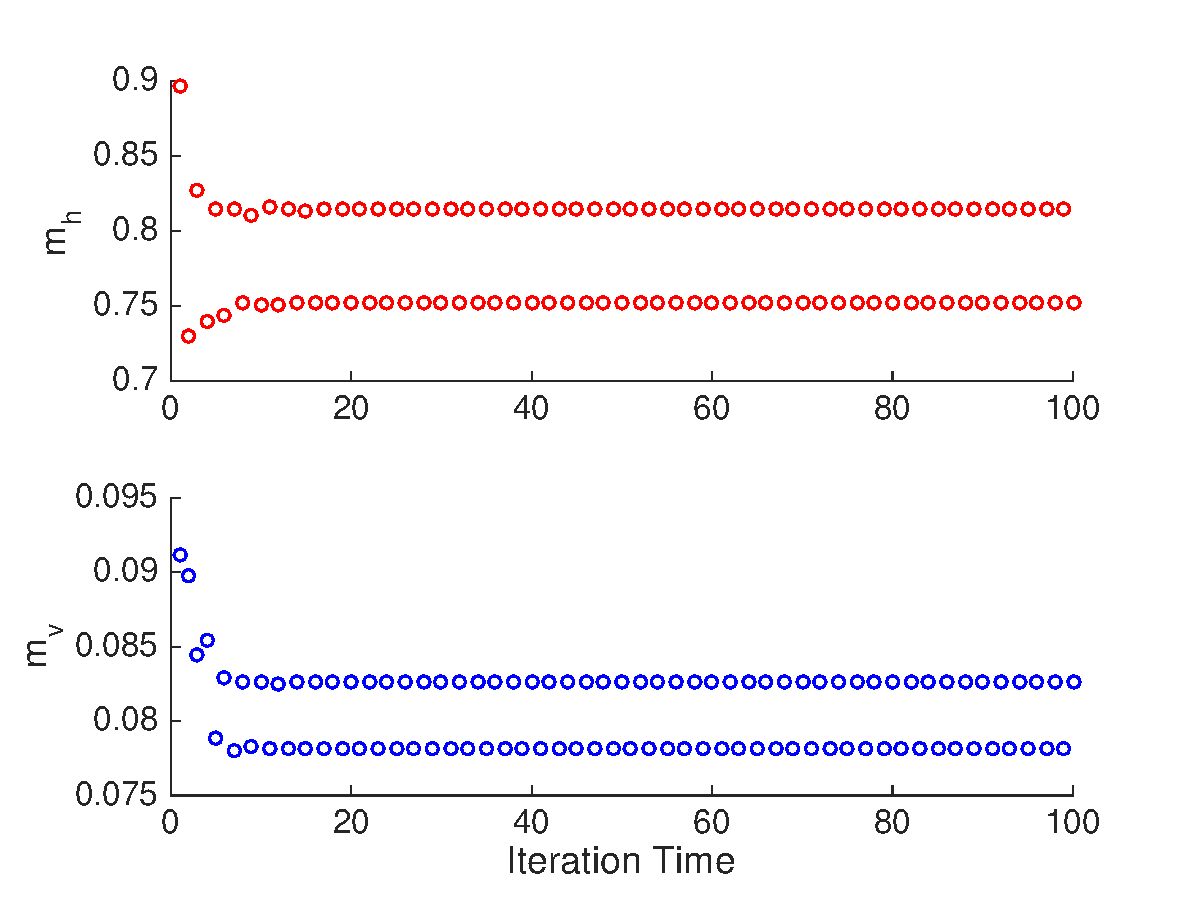
\includegraphics[width=0.48\textwidth]{figure/TAP_results/mvmh_20.eps}}
	\subfigure{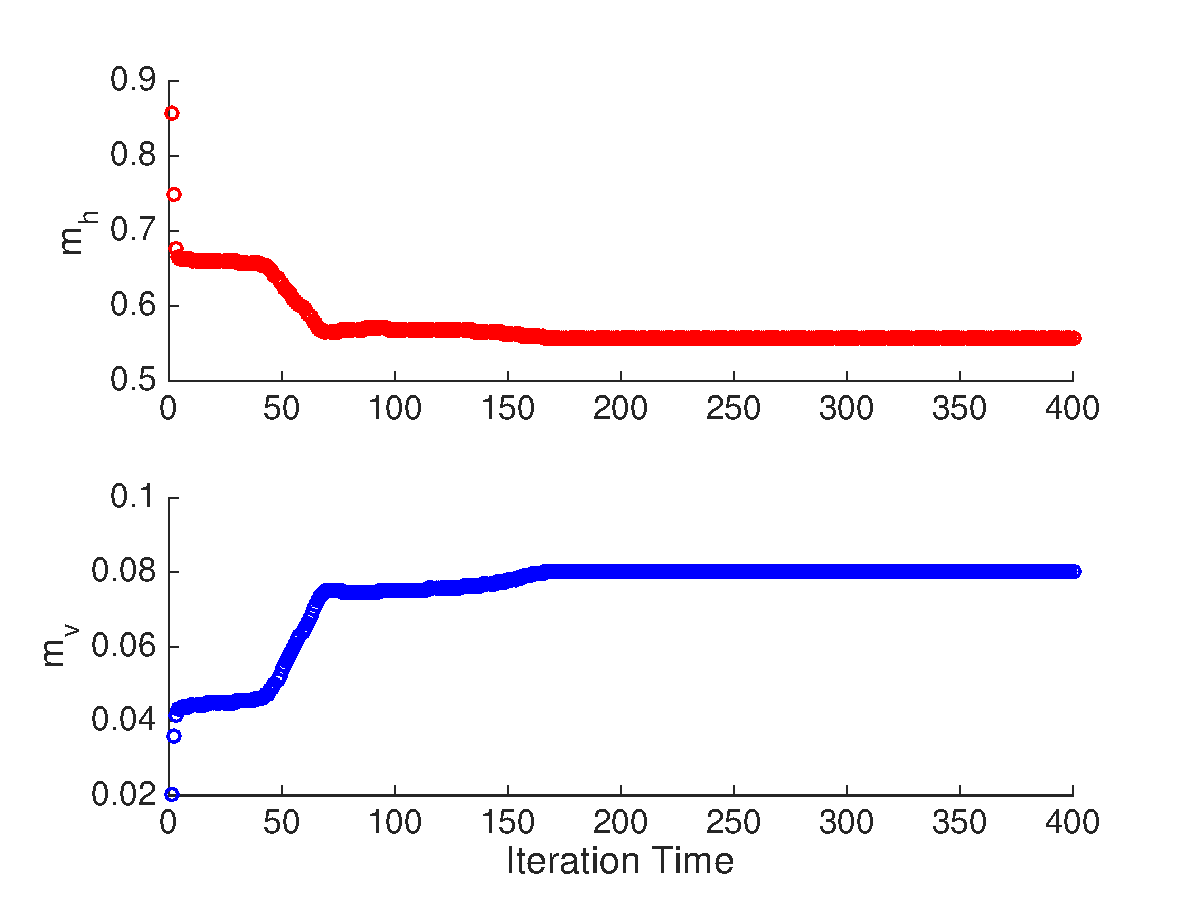
\includegraphics[width=0.48\textwidth]{figure/TAP_results/mvmh_100.eps}}
	\subfigure{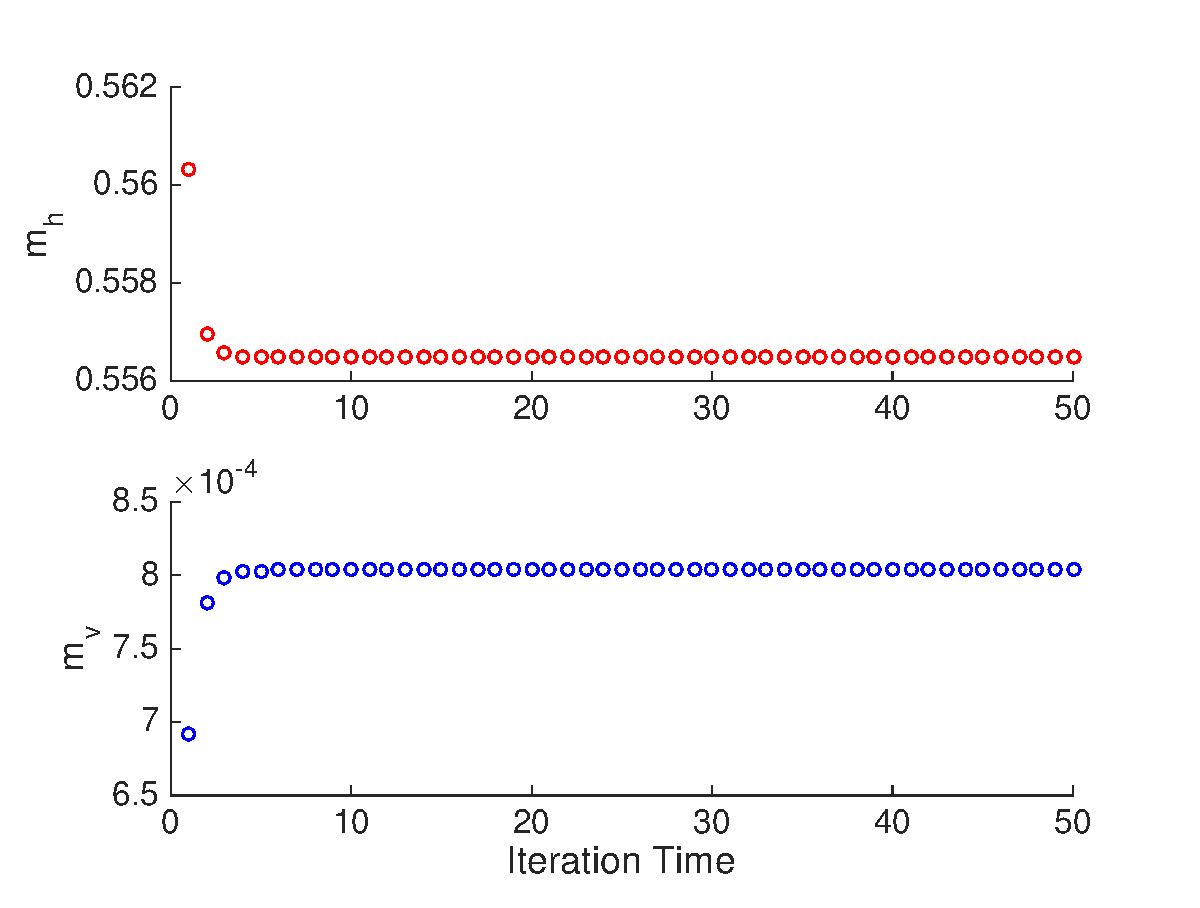
\includegraphics[width=0.48\textwidth]{figure/TAP_results/mvmh_500.eps}}
% \vspace{-0.1in}
\caption{$m_{h}$, $m_{v}$ convergence condition using TAP method. From left to right, up to down, the figure indicates an RBM model with 10, 20, 100, 500 hidden units. The convergence time is approximately 40, 20, 175, 5. By such few iteration time, all results can be obtained in less than 1 second.}
\label{fig:TAPmhmviter} % FIG1
\end{minipage}
\vspace{-0.05in}
\end{figure}
When running a TAP, we see we can get converged $m_{v}$ \& $m_{h}$ in very few iteration time (Figure~\ref{fig:TAPmhmviter}, convergence time is approximately 40, 20, 175, 5 for the model with 10, 20, 100, 500 hidden units respectively). Given this observation, the computing time of TAP is negligeable (we obtain all results in less than a second). And also, its meaningless to discuss standard deviation here.

However, we do notice that the converged results are sometimes not consistent but periodic. (eg. Figure~\ref{fig:TAPmhmviter}, when there are 10, 20 hidden units), this is not a good news because even if we have more resources to compute the iterations, we would not have a better result.

\begin{table}[t]
\centering
{\small
\begin{tabular}{c|ccccc}
    \hline
    \textbf{Hid Units} & \textbf{TAP} & \textbf{AIS} & \textbf{RTS} & \textbf{Real Value} \\ 
    \hline
	   10  & 212.32 & 226.05 & 226.2707 & 226.11 	  \\
	   20  & 214.85 & 221.11 & 218.8993 & N/A 	  \\
	   100 & 342.02 & 348.45 & 347.3684 & N/A 	  \\
	   500 & 450.31 & 463.25 & 459.7372 & N/A 	  \\ \hline
\end{tabular}
}
\vspace{-0.1in}
\caption{$Z(\theta)$ estimation result of TAP, AIS, RTS (AIS \& RTS with $\mathbf b$ init)}
\label{tab:allresult}
% \vspace{-0.05in}
\end{table}
\begin{table}[t]
\centering
{\small
\begin{tabular}{c|ccccc}
    \hline
    \textbf{Hid Units} & \textbf{TAP} & \textbf{AIS} & \textbf{RTS} \\ 
    \hline
	   10  & < 1 & 77.38 & 68.28  \\
	   20  & < 1 & 63.03 & 87.42  \\
	   100 & < 1 & 92.87 & 164.34 \\
	   500 & < 1 & 154.63 & 603.59 \\ \hline
\end{tabular}
}
\vspace{-0.1in}
\caption{Efficiency of TAP, AIS, RTS (Unit: seconds), with a Intel Core i5 CPU Turbo Boost to 2.7GHz}
\label{tab:efficiencyresult}
% \vspace{-0.05in}
\end{table}

And disappointingly, compared to the result of other algorithms (Table~\ref{tab:allresult}), TAP usually have a lower estimation value, which is not preferable.









%!TEX root = RBM.tex


\subsection{Theoretical Anaylsis}

% Since TAP's result is relatively irrelevant to the run time and resources. We use the value estimated in the last subsection.

% \subsubsection{Practice}
% \para{Complexity}
% For horizontal comparison on complexity, we let the correctness \& stability to be approximately the same (i.e. the correctness the AIS could achieve in 2 seconds), and compare the run time for three algorithms.

% We have conducted 20 experiments for the acquistion of $Z(\theta)$.

% From our practice, we have found that xxx gives the most agreeable result while TAP completely underestimate the value.


% \para{Correctness \& Stability}
% For horizontal comparison on the correctness \& stability, we allow the same run time for AIS and RTS algorithms to compute (i.e. 10 seconds per experiment). We have conducted 20 experiments for the acquistion of $Z(\theta)$.

% From our practice, we have found that xxx gives the most agreeable result while TAP completely underestimate the value.

% We also notice that the variance of ... is the smallest which indicates it has the best stability.


\para{RTS}
From a theretical perspective, we have proven that the bias \& the variance of the RTS method are to be:
\begin{equation}
E{[ log \hat{Z}_{k}^{RTS} ]} - E{[Z_{k}]} \approx \frac{1}{2}{[\frac{\sigma^{2}_{1}}{\hat{c}^{2}_{1}}-\frac{\sigma^{2}_{k}}{\hat{c}^{2}_{k}}]} 
\end{equation}
\begin{equation}
Var{[ log \hat{Z}_{k}^{RTS} ]} \approx \frac{\sigma^{2}_{1}}{\hat{c}^{2}_{1}} + \frac{\sigma^{2}_{k}}{\hat{c}^{2}_{k}} - \frac{2\sigma_{1k}}{\hat{c}_{k}\hat{c}_{1}}
\end{equation}
where $\sigma^{2}_{k} = Var{[\hat{c}_{k}]}$ and $\sigma_{1k} = Cov{[\hat{c}_{1},\hat{c}_{k}]}$

This has shown that the bias of RTS has no definite sign.

\para{AIS}
However, in AIS, Neal and Jarzynski et al.\cite{neal2001annealed,nonequilibrium} have shown that if we want the result to be unbiased, we would have to let $M=1$ in the iteration, which by doing so have lost the advantage of AIS. That is to say, on the other hand, if $M > 1$, we would have a negative bias due to Jenson Inequality.

From the result of our practice, we see when AIS and RTS show same good performance in estimation, RTS's efficiency is a little bit lower than that of AIS's.

\para{TAP}
Although TAP shows the best efficiency, its results are the most disapointing. Apparantly TAP has underestimate the value of the partition function.

We did not analyze deeply on the reasons why it failed to perform a satisfying result, but our intuition tells that maybe it is because the Legendre transform. In our practice, we only took the Legendre transform to the 2nd order, which might result in the underestimation.











